%===============================================================================
%============ Good Thoughts, Good Words, Good Deeds ============
%===============================================================================
% Template:     Premium LaTeX Resume Template (Persian & English)
% Author:       Mahdi Jahangiri (Open Source Contributor)
% GitHub:       https://github.com/MahdiJahangiry/Premium-Persian-CV
% License:      MIT License
% Description:  A highly customizable, single-page, ATS-friendly LaTeX resume 
%               template with 8 premium color palettes and XePersian support.
% ==============================================================================


\documentclass[10pt,a4paper]{article}

% Page margins optimized for LTR single-page layout
\usepackage[left=0.75cm, right=1.5cm, top=1.2cm, bottom=1cm]{geometry}
\usepackage{xcolor}
\usepackage{tikz}
\usepackage{eso-pic}
\usepackage{fontawesome5}
\usepackage{enumitem}
\usepackage{graphicx}
\usepackage{setspace}
\usepackage[hidelinks]{hyperref}

% Modern Sans-Serif Font setup for English
\renewcommand{\familydefault}{\sfdefault}
\usepackage[T1]{fontenc}

% ==========================================
% Custom Color Palettes
% Uncomment the desired palette block to use it
% ==========================================

% --- Palette 1: Sage Green (Active) ---
\definecolor{sidebarbg}{HTML}{C8DBCF} 
\definecolor{sidebartitle}{HTML}{144517} 
\definecolor{sidebartext}{HTML}{1F6322} 
\definecolor{accent}{HTML}{009E3A} 
\definecolor{primary}{HTML}{111111} 

% --- Palette 2: Dark Pine & Mint ---
% \definecolor{sidebarbg}{HTML}{0E2922} 
% \definecolor{sidebartitle}{HTML}{FFFFFF} 
% \definecolor{sidebartext}{HTML}{B3D4C8} 
% \definecolor{accent}{HTML}{00E676} 
% \definecolor{primary}{HTML}{0E2922} 

% --- Palette 3: Dark Olive & Matte Gold ---
% \definecolor{sidebarbg}{HTML}{3A4032} 
% \definecolor{sidebartitle}{HTML}{F9F6EE} 
% \definecolor{sidebartext}{HTML}{D1D7C1} 
% \definecolor{accent}{HTML}{D4AF37} 
% \definecolor{primary}{HTML}{222222} 

% --- Palette 4: Emerald Slate & Turquoise ---
% \definecolor{sidebarbg}{HTML}{1B3B36} 
% \definecolor{sidebartitle}{HTML}{E0F2F1} 
% \definecolor{sidebartext}{HTML}{80CBC4} 
% \definecolor{accent}{HTML}{1DE9B6} 
% \definecolor{primary}{HTML}{1B3B36} 

% --- Palette 5: Oxford Navy & Camel (MBA Classic) ---
%\definecolor{sidebarbg}{HTML}{1B263B} 
%\definecolor{sidebartitle}{HTML}{E0E1DD} 
%\definecolor{sidebartext}{HTML}{778DA9} 
%\definecolor{accent}{HTML}{D4A373} 
%\definecolor{primary}{HTML}{1B263B} 

% ------------------------------------------
% Standard Text Colors
\definecolor{graytext}{HTML}{444444} 
\definecolor{lightgray}{HTML}{E0E0E0} 
% ==========================================

% Custom Bullet Points
\newcommand{\mybullet}{\tikz[baseline=-0.6ex]\draw[accent,fill=accent] (0,0) circle (1.5pt);}

% Section Title Styling (Main Column)
\newcommand{\cvmainsect}[1]{
	\vspace{1.5mm}
	\noindent{\Large\bfseries\textcolor{primary}{#1}}
	\vspace{1mm}\par
	\noindent\textcolor{lightgray}{\rule{\linewidth}{1pt}}\par
	\vspace{1.5mm}
}

% Section Title Styling (Sidebar)
\newcommand{\cvsidebarsect}[1]{
	\vspace{4mm}
	\noindent{\large\bfseries\textcolor{sidebartitle}{#1}}
	\vspace{1mm}\par
	\noindent\textcolor{sidebartitle!40}{\rule{\linewidth}{0.5pt}}\par
	\vspace{2mm}
}

% Resume Entry Macro (Job/Education)
\newcommand{\resumeentry}[4]{
	\noindent\textbf{\textcolor{primary}{#1}} \hfill \textcolor{accent}{\footnotesize \faCalendar\quad #2} \\
	\noindent\textcolor{graytext}{\textit{\small #3}} \hfill \textcolor{graytext}{\textit{\footnotesize \faMapMarker*\quad #4}} \par\vspace{1mm}
}

% Sidebar Skill Bars Macro
\newcommand{\sidebarskill}[2]{
	\noindent{\footnotesize\textcolor{sidebartext}{#1}} \hfill
	\begin{tikzpicture}[baseline=-0.5ex]
		\draw[fill=sidebartitle!15, draw=none, rounded corners=0.5pt] (0,0) rectangle (2.2, 0.12);
		\draw[fill=accent, draw=none, rounded corners=0.5pt] (0,0) rectangle ({2.2 * #2 / 100}, 0.12);
	\end{tikzpicture}\par\vspace{1mm}
}

% Sidebar Soft Skills Rating Macro
\newcommand{\softskill}[2]{
	\noindent{\footnotesize\textcolor{sidebartext}{#1}} \hfill
	\begin{tikzpicture}[baseline=-0.5ex]
		\foreach \x in {1,...,5} {
			\ifnum\x>#2
			\draw[fill=sidebartitle!15, draw=none] (\x*0.35,0) circle (1.5pt);
			\else
			\draw[fill=accent, draw=none] (\x*0.35,0) circle (1.5pt);
			\fi
		}
	\end{tikzpicture}\par\vspace{1mm}
}

% Draw Sidebar Background (Adjusted for Left Side in LTR)
\AddToShipoutPictureBG{%
	\begin{tikzpicture}[remember picture, overlay]
		\fill[sidebarbg] (current page.north west) rectangle ++(7.5cm, -29.7cm);
	\end{tikzpicture}
}

\begin{document}
	\pagestyle{empty}
	
	% ==========================================
	% Left Sidebar Column
	% ==========================================
	\noindent
	\begin{minipage}[t]{6cm}
		\vspace*{0pt}
		
		% Profile Picture
		\begin{center}
			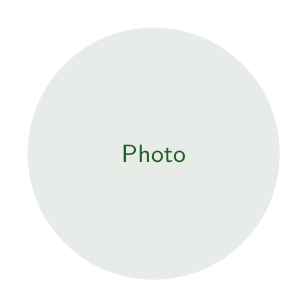
\begin{tikzpicture}
				% Placeholder for missing image. Delete this line if using a real image.
				 \draw[fill=sidebartitle!10, draw=none] (0,0) circle (1.6cm) node {\small \textcolor{sidebartext}{Photo}};
				
				% Uncomment the 2 lines below and add your photo (e.g., photo.jpg) to the folder
%				\clip (0,0) circle (1.6cm);
%				\node at (0,0) {\includegraphics[width=3.2cm]{./photo.jpg}};
			\end{tikzpicture}
		\end{center}
		
		\vspace{1.5mm}
		
		% Name and Job Title
		\begin{center}
			{\LARGE \textbf{\textcolor{sidebartitle}{[First Name] [Last Name]}}}\\[2.5mm]
			{\footnotesize \textbf{\textcolor{accent}{[Your Professional Title / e.g. Operations Analyst]}}}
		\end{center}
		
		% Contact Information
		\cvsidebarsect{Contact}
		\noindent\textcolor{accent}{\small \faMapMarker*} \quad \textcolor{sidebartext}{\footnotesize [City, Country]} \par\vspace{1.5mm}
		\noindent\textcolor{accent}{\small \faPhone} \quad \textcolor{sidebartext}{\footnotesize [+1 234 567 890]} \par\vspace{1.5mm}
		\noindent\textcolor{accent}{\small \faEnvelope} \quad \href{mailto:your.email@example.com}{\textcolor{sidebartext}{\footnotesize your.email@example.com}} \par\vspace{1.5mm}
		\noindent\textcolor{accent}{\small \faLinkedin} \quad \href{https://linkedin.com/in/YourUsername}{\textcolor{sidebartext}{\footnotesize linkedin.com/in/YourUsername}} \par\vspace{1.5mm}
		\noindent\textcolor{accent}{\small \faGithub} \quad \href{https://github.com/YourUsername}{\textcolor{sidebartext}{\footnotesize github.com/YourUsername}} \par\vspace{1.5mm}
		
		% Hard Skills
		\cvsidebarsect{Hard Skills}
		\sidebarskill{Skill Name 1}{90}
		\sidebarskill{Skill Name 2}{80}
		\sidebarskill{Skill Name 3}{70}
		\sidebarskill{Skill Name 4}{100}
		\sidebarskill{Skill Name 5}{60}
		
		% Soft Skills
		\cvsidebarsect{Soft Skills}
		\softskill{Soft Skill 1}{5}
		\softskill{Soft Skill 2}{4}
		\softskill{Soft Skill 3}{5}
		\softskill{Soft Skill 4}{4}
		\softskill{Soft Skill 5}{3}
		
	\end{minipage}%
	\hspace{1.25cm}%
	% ==========================================
	% Right Main Column
	% ==========================================
	\begin{minipage}[t]{11.5cm}
		\vspace*{0pt}
		
		% Executive Summary
		\cvmainsect{Executive Summary}
		\setstretch{1.55} 
		\footnotesize \textcolor{graytext}{
			[Write a strong, one-paragraph summary of your expertise, experience, and career goals here. Focus on the value you bring to an organization, avoiding clichés. Highlight your core technical skills and practical experiences. This section should immediately convince the hiring manager to read the rest of your resume.]
		}
		
		\vspace{1.5mm}
		
		% Work Experience
		\cvmainsect{Work Experience}
		
		\resumeentry{[Recent Job Title]}{[Start Year] -- Present}{[Company Name]}{[City, Country]}
		\vspace{-1.5mm}
		\begin{itemize}[leftmargin=*, label={\mybullet}, nosep, itemsep=2pt]
			\item \footnotesize\textcolor{graytext}{[Describe your first major achievement: managing processes, increasing sales, or solving technical issues.]}
			\item \footnotesize\textcolor{graytext}{[Describe your second achievement: using specific tools or communicating with clients.]}
		\end{itemize}
		
		\vspace{1.5mm} 
		
		\resumeentry{[Previous Job Title]}{[Start Year] -- [End Year]}{[Company Name]}{[City, Country]}
		\vspace{-1.5mm}
		\begin{itemize}[leftmargin=*, label={\mybullet}, nosep, itemsep=2pt]
			\item \footnotesize\textcolor{graytext}{[Describe your primary responsibility or accomplishment in this role.]}
			\item \footnotesize\textcolor{graytext}{[Describe a secondary responsibility and its impact on the organization.]}
			\item \footnotesize\textcolor{graytext}{[Add a third point if necessary to highlight specific tools or methodologies used.]}
		\end{itemize}
		
		% Education
		\cvmainsect{Education}
		\resumeentry{[Degree Name e.g. Master of Business Administration]}{[Graduation Year]}{[University/Institution Name]}{[City, Country]}
		\vspace{-1.5mm}
		\begin{itemize}[leftmargin=*, label={\mybullet}, nosep]
			\item \footnotesize\textcolor{graytext}{\textbf{Thesis/Research Topic:} [Enter your main research topic or thesis title here.]}
		\end{itemize}
		
		% Projects & Technical Experience
		\cvmainsect{Projects \& Technical Experience}
		
		\begin{itemize}[leftmargin=*, label={\mybullet}, nosep, itemsep=2pt]
			\item \footnotesize\textcolor{graytext}{\textbf{[Project Title 1]:} [Briefly explain the tools, frameworks, and methodologies used in this project.]}
			
			\item \footnotesize\textcolor{graytext}{\textbf{[Project Title 2]:} [Describe your role in developing, implementing, or optimizing systems.]}
			
			\item \footnotesize\textcolor{graytext}{\textbf{[Project Title 3]:} [Mention the final outcome or the business value created by this project.]}
		\end{itemize}
		
		% Certifications & Additional Info
		\cvmainsect{Certifications \& Additional Info}
		\noindent\begin{minipage}[t]{0.48\textwidth}
			\vspace{0pt}
			\textbf{\textcolor{primary}{\small Certifications}}\\[1.5mm]
			\footnotesize \textbf{[Course Name 1]} \quad \textcolor{graytext}{\scriptsize ([Issue Date])} \\
			\textcolor{graytext}{\scriptsize \textit{[Issuing Organization]}} \\[2mm]
			\footnotesize \textbf{[Course Name 2]} \quad \textcolor{graytext}{\scriptsize ([Issue Date])} \\
			\textcolor{graytext}{\scriptsize \textit{[Issuing Organization]}}
		\end{minipage}\hfill
		\begin{minipage}[t]{0.48\textwidth}
			\vspace{0pt}
			\textbf{\textcolor{primary}{\small Personal Information}}\\[1.5mm]
			\footnotesize\textcolor{graytext}{\textbf{Date of Birth:} [YYYY] \quad|\quad \textbf{Status:} [e.g., Single]} \\[2.5mm]
			\textbf{\textcolor{primary}{\small References:}} \\
			\footnotesize\textcolor{graytext}{\textbf{[Reference Name]} ([Reference Job Title])} \\
			\footnotesize\textcolor{graytext}{\faEnvelope \ \href{mailto:ref@example.com}{ref@example.com}}
		\end{minipage}
		
	\end{minipage}
	
\end{document}